\chapter*{Serie 1}
\section*{Exercise 1}
\subsection*{Backward Euler update formula derivation}
General update formula
\begin{equation}
 y_{k+1} = y_k + \rd t \cdot f(t_{k+1}, y{k+1})
\end{equation}

In concrete terms for the equations of motion, it is
\begin{subequations}
 \begin{align}
  x_{k+1} &= x_k + \rd t \cdot v_{k+1}
  \label{eq:xkp1}\\
  v_{k+1} &= v_k + \rd t \cdot \left( \frac{k(-x_{k+1} -L)}{m} - \frac{d\cdot v_{k+1}}{m} -g \right)
  \label{eq:vkp1}
 \end{align}
\end{subequations}
Insert \eqref{eq:xkp1} into \eqref{eq:vkp1} and reorder.
\begin{subequations}
 \begin{align}
  v_{k+1} &= v_k + \rd t \cdot \left( \frac{k(-x_{k+1} -L)}{m} - \frac{d\cdot v_{k+1}}{m} -g \right)\\
          &= \rd t\left(-\frac{k}{m}\rd t - \frac{d}{m}\right) v_{k+1} + v_k + \rd t\left( \frac{k}{m}(-x_k-L)-g \right)\\
          &= \frac{ v_k -\rd t \left(\frac{k}{m} (x_k + L) -g \right)}{1+\rd t \left( \frac{k\cdot \rd t + d}{m} \right)}
 \end{align}
\end{subequations}
\section*{Exercise 2}
\subsection*{2.1. Analytic solution}
First lets do a sketch as seen in figure \ref{fig:sp} to omit any misunderstanding of the problem.
\begin{figure}[]
	\begin{center}
		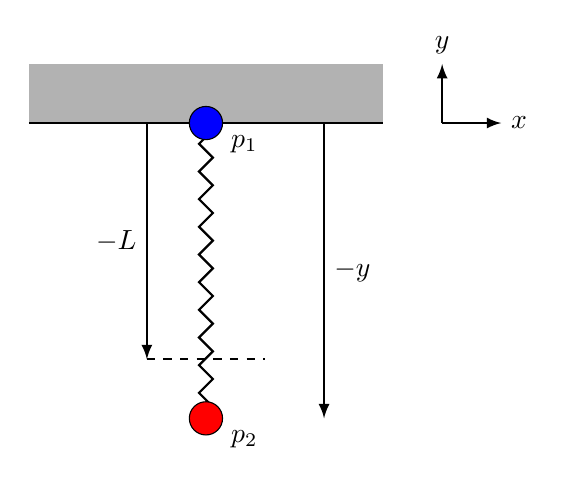
\begin{tikzpicture}[decoration=zigzag, mass/.style={label distance=2mm},scale=1.5]
			\fill[black!30] (-1.5,0) rectangle (1.5,0.5);
			\draw[thick] (-1.5,0) -- (1.5,0);
			\begin{scope}[shift={(2,0)}]
				\coordinate[label=above:$y$,thick] (y) at (0,0.5);
				\coordinate[label=right:$x$,thick] (x) at (0.5,0);
				\draw[-latex,thick] (0,0) -- (y);
				\draw[-latex,thick] (0,0) -- (x);
			\end{scope}
			\coordinate[label={[mass]350:$p_1$}] (m1) at (0,0);
			\coordinate[label={[mass]350:$p_2$}] (m2) at (0,-2.5);
			\draw[decorate,thick] (m1) -- (m2);
			\fill[blue,draw=black] (m1) circle (4pt);
			\fill[red,draw=black] (m2) circle (4pt);
			\path[-latex,draw,thick] (-0.5,0) to[left] node{$-L$} (-0.5,-2);
			\path[-latex,draw,thick] (1,0) to[right] node{$-y$} (1,-2.5);
			\draw[dashed,thick] (-0.5,-2) -- (0.5,-2);
		\end{tikzpicture}
	\end{center}
	\caption{Sketch of the spring problem, $p_2$ being not in rest state.}
	\label{fig:sp}
\end{figure}
We would like to find the constants $c_1, c_2$ of the equation
\begin{align}
	y(t)&=c_1 e^{\alpha t}\cos (\beta t)+c_2 e^{\alpha t}\sin(\beta t) - L -\frac{mg}{k},
	\label{eq:gf}
	\intertext{where the constraints are the rest state initial conditions, which means there is no energy in the system except gravitational energy at $t=0$. This has the same physical meaning as the spring having its rest length $L$ \footnote{if there would be no other force than the one of the feather} and no kinetic energy at $t=0$. This can be expressed as}
	 y(t=0) &= -L,
	\label{eq:c1a}
	\shortintertext{and}
		\dot{y}(t=0)&=0.
	\label{eq:c2a}
	 \intertext{The position of $p_2$ computed with the given solution Eq. \ref{eq:gf} is}
	 y(t=0) &= c_1-L-\frac{mg}{k}.
	\label{eq:c1b}
	\intertext{Comparing Eq. \ref{eq:c1a} and Eq. \ref{eq:c1b} gives us}
	c_1&=\frac{mg}{k}.
	\intertext{To get $c_2$ we need to compute $\dot{y}(t=0)$ from  Eq. \ref{eq:gf}}
	\dot{y}(t=0)&=\!\left( c_1\alpha +c_2 \beta -L -\frac{mg}{k} \right),
	\shortintertext{where $c_1=mg/k$ leads to}
	\dot{y}(t=0)&= \frac{mg}{k}\alpha +c_2\beta -L-\frac{mg}{k}.
	\intertext{Using the constraint in Eq. \ref{eq:c2a} finally gives us}
	c_2&=\frac{mg}{\beta k}(1-\alpha)+\frac{L}{\beta}.
\end{align}
\subsection*{2.2. Error convergence analysis}
The error convergence plots are all quite similar with respect to different damping factors. The three Euler methods show the lowest average error convergence, in comparison to the Midpoint method. This is what we expect, since the Midpoint method is known to be accurate of order 2, while Euler methods are only accurate of order 1.

In concrete terms, the following values for the error convergence $\frac{e_{i+1}}{e_i}$ (damping factor 0) were obtained.

\begin{tabular}{ll}
Euler			& 3.89\\
Symplectic Euler	& 4.10\\
Backwards Euler		& 3.84\\
Midpoint		& 9.57\\
\end{tabular}

In order to get meaningful results, the first three measurements were ignored when computing the average error convergence.


\begin{figure}[h]
	\centering
	\subfloat[damping factor $d=0.01$]{
		\includegraphics*[width=0.8\textwidth]{../data/ex1/errorConvergenceDamp0_01-crop.pdf}
	\label{fig:errorconvd001} 
}
\end{figure}
\begin{figure}
	\ContinuedFloat
	\centering
\subfloat[damping factor $d=0$]{
		\includegraphics*[width=0.8\textwidth]{../data/ex1/errorConvergenceDamp0-crop.pdf}
}%
	\label{fig:errorconvd0} 
\end{figure}
\begin{figure}
	\ContinuedFloat
	\centering
\subfloat[damping factor $d=1$]{
		\includegraphics*[width=0.8\textwidth]{../data/ex1/errorConvergenceDamp1-crop.pdf}
	}%
	\label{fig:errorconvd1} 
\end{figure}

\subsection*{2.3. Stability analysis}
As expected, the backwards Euler method is unconditionally stable. The symplectic Euler method is also stable, which was pointed out during the lecture. Both midpoint and Euler method are not stable, which is also as expected.

However, for a damping coefficient of 1.9, all methods seem to be stable. But for a general setting, the Midpoint and Euler method remain unstable.

Since an accurate method produces a smaller error per step, the error propagation is smaller, therefore it is more likely to be stable.

\begin{figure}[h]
	\centering
	\subfloat[damping factor $d=0$]{
		\includegraphics*[width=0.8\textwidth]{../data/ex1/stabilityMeasurementDamp0-crop.pdf}
	\label{fig:stabanald0} 
}
\end{figure}
\begin{figure}
	\ContinuedFloat
	\centering
\subfloat[damping factor $d=1.9$]{
		\includegraphics*[width=0.8\textwidth]{../data/ex1/stabilityMeasurementDamp1_9-crop.pdf}
}%
	\label{fig:stabanald19} 
\end{figure}

one may want to plot ‘dof’ versus ‘L2’ or ‘dof’ versus ‘Lmax’. This can be done by
\begin{tikzpicture}
	\begin{loglogaxis}[
			xlabel=Dof,
		ylabel=$L_2$ error]
		%\addplot table[x=step,y=euler] {datafile.dat};
	\end{loglogaxis}
\end{tikzpicture}
